% set figure directory
\graphicspath{{../graph_nn/fig/}}
\section{使用图神经网络进行半监督分类}
在上一节中,我们使用了谱聚类和SBM模型对Mathlib4中的数学定理和证明进行了社群识别,并使用modularity、ARI和NMI指标对得到的社群结果进行了评价。从较低的ARI和NMI指标可以看出,我们社群发现的结果相较于按学科进行划分的结果有明显的差异;而从比学科划分更高的modularity指标来看,有理由认为社群发现的结果相较单纯的学科划分更能体现出数学概念之间的逻辑关系。

尽管谱聚类和SBM模型对于数据的社群发现可能提供了学科划分之外新的视角,但是两种方法作为无监督的学习方法,较低的可解释性和较大的评估难度是其固有的缺陷。

在本节中,我们将以每个节点的学科作为标签,使用图神经网络(GNNs)对Mathlib4中的数学定理和证明进行半监督分类。并将模型在测试集上的表现与按学科分类的真实结果进行对比。

\subsection{\texttt{PyTorch}数据准备}
我们使用\texttt{PyTorch Geometric}库来进行图卷积神经网络(GCNs)的构建和训练。为此,我们需要将Mathlib4中的数据转换为\texttt{PyTorch Geometric}中的\texttt{Data}对象,该对象包含了图的结构信息和节点特征信息。具体来说,包括:
\begin{itemize}
    \item \texttt{x}:节点特征矩阵,每一行代表一个节点的特征向量;
    \item \texttt{edge\_index}:边的索引矩阵,每一列代表一条边的起始节点和终止节点的索引;
    \item \texttt{y}:节点标签向量,每一个元素代表一个节点的标签;
    \item \texttt{train\_mask}:训练集掩码向量,每一个元素代表一个节点是否在训练集中(\texttt{val\_mask}和\texttt{test\_mask}同理)。
\end{itemize}

关于节点特征矩阵\texttt{x},因为我们分类仅仅用到的是图的依赖结构,节点特征并不包含额外的信息,我们该如何初始化节点特征矩阵是一个值得考虑的问题。一个简单的想法可能是赋予每个节点相同的特征向量,如\texttt{x}为全零或全一向量。然而这样的初始化使得模型没有办法学习到有用的信息;回头考虑GCN的结构不难发现,这样的初始化使得模型不能够区分不同的节点。对此,一个简单的改进是将\texttt{x}初始化为单位矩阵。值得注意的是,其他可以考虑的选择包括使用Laplacian矩阵的特征向量作为节点特征,或者使用预训练的embedding作为节点特征。

关于图的边索引矩阵\texttt{edge\_index},我们将Mathlib4中的依赖关系作为无向边处理。为了适应GCN的结构,这一简化处理损失了依赖关系的方向性,尽管在数学证明的范畴下这一简化可能是合理的。然而,可能的改进方向包括使用自然考虑到图的方向性的模型如Graph Attention Networks(GATs)。

关于节点标签向量\texttt{y},我们将每个节点的学科作为标签。由于\texttt{Torch}期望标签是从0开始的整数,我们将学科的字符串标签映射到整数标签。

关于训练-验证-测试集的划分,我们选取三者的比例为$8:1:1$,并使用掩码向量做出标记。

\subsection{构建GCN模型并训练}
我们使用\texttt{PyTorch Geometric}库中的\texttt{GCNConv}层来构建GCN模型。我们的模型初步包括两层GCN层,后接一个ReLU激活函数,最后以类别数大小的线性层输出。我们使用交叉熵损失函数和Adam优化器进行训练,注意到\texttt{Torch}中的交叉熵损失函数会自动将Softmax函数作用于线性输出层。

模型可以调整的超参数包括GCN的层数、隐藏层的维度、学习率、epoch数等。通过观察模型在验证集上的表现,我们调整模型为一层GCN,隐藏层维度为512,学习率为0.01,epoch数为30。模型的训练曲线如图\ref{fig:gcn_train}所示。% loss曲线和accuracy曲线

\begin{figure}[htbp]
    \centering
    \begin{subfigure}{0.48\textwidth}
        \centering
        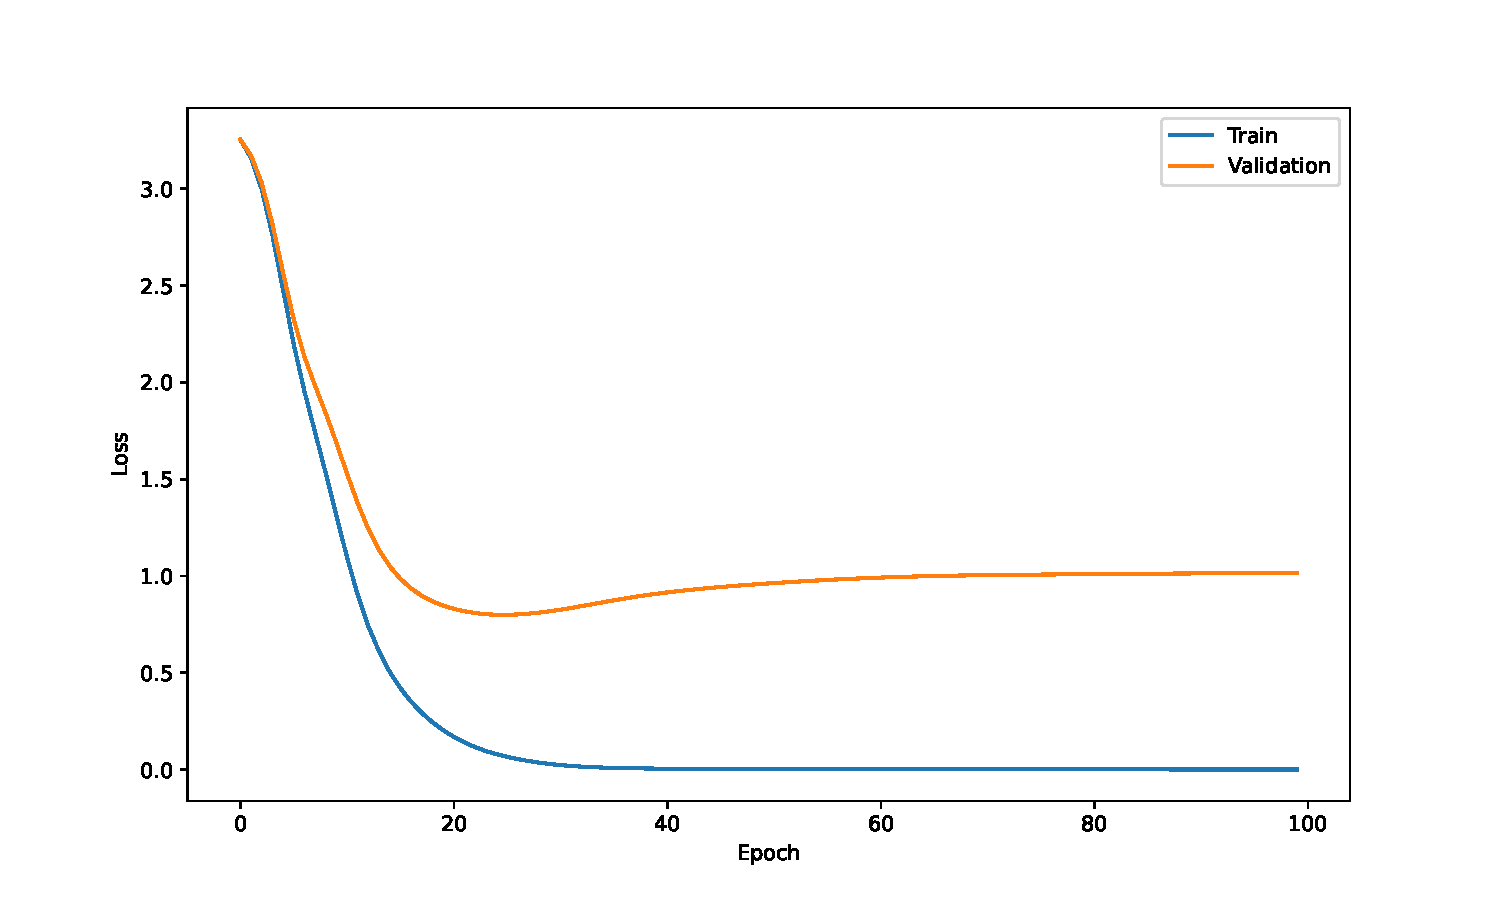
\includegraphics[width=\textwidth]{loss.pdf}
        \caption{Loss曲线}
    \end{subfigure}
    \begin{subfigure}{0.48\textwidth}
        \centering
        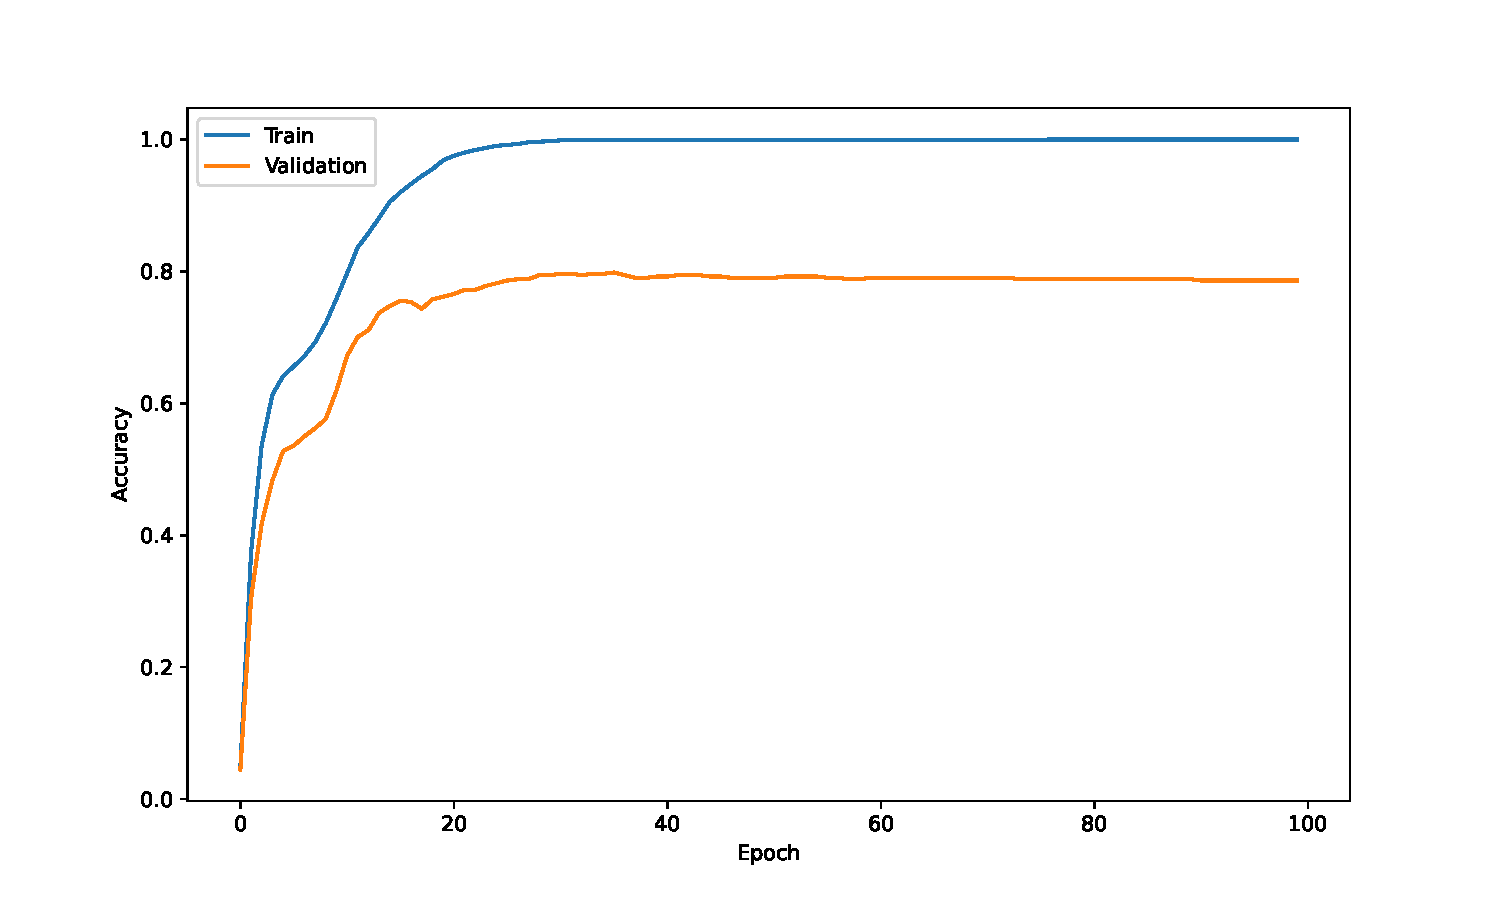
\includegraphics[width=\textwidth]{acc.pdf}
        \caption{Accuracy曲线}
    \end{subfigure}
    \caption{GCN模型训练曲线}
    \label{fig:gcn_train}
\end{figure}

\subsection{模型评估}
我们使用模型在测试集上的准确率和混淆矩阵来评估模型的性能。同时,一个容易想到的Baseline模型是将每个节点的邻居标签众数表决的结果作为预测结果。二者在测试集上的准确率对比如表\ref{tab:gcn_acc}所示。二者的预测结果的混淆矩阵对比如表\ref{tab:gcn_confusion}所示。

\begin{table}[htbp]
    \centering
    \caption{GCN模型和Baseline模型在测试集上的准确率}
    \begin{tabular}{cc}
        \toprule
        模型 & 准确率 \\
        \midrule
        Baseline & 56.01\% \\
        GCN & 76.58\% \\
        \bottomrule
    \end{tabular}
    \label{tab:gcn_acc}
\end{table}

\begin{figure}
    \centering
    \begin{subfigure}{0.48\textwidth}
        \centering
        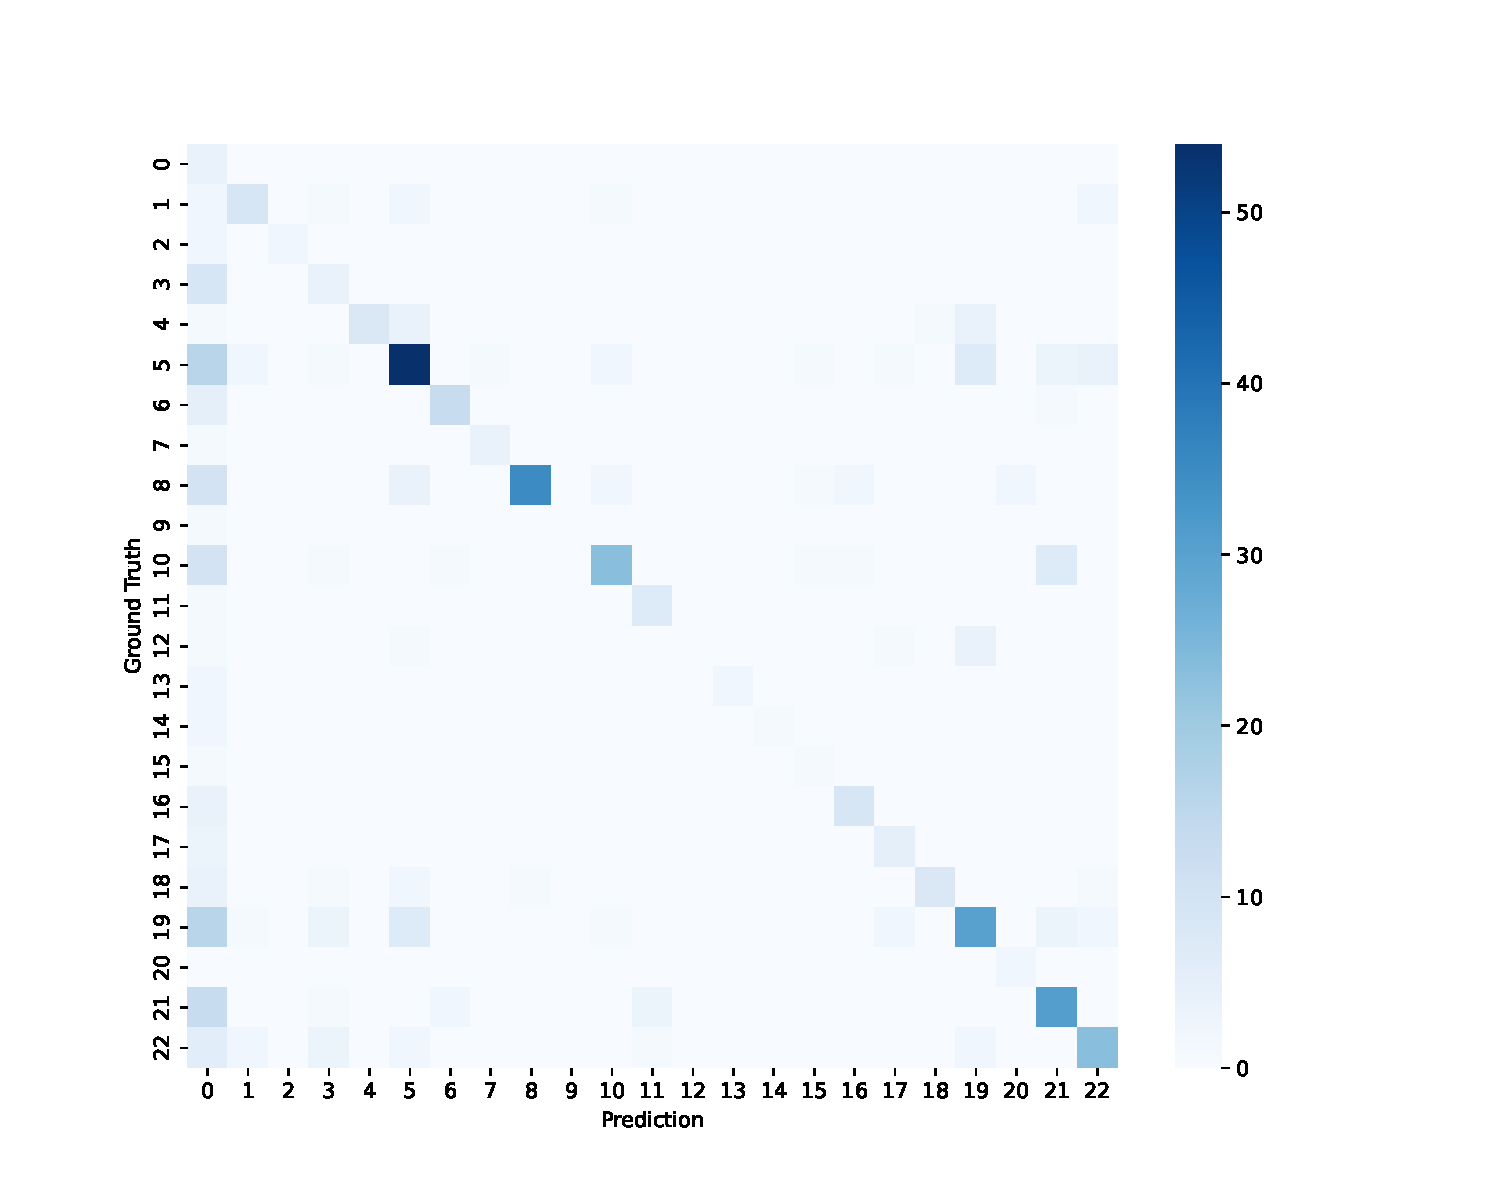
\includegraphics[width=\textwidth]{confusion_matrix_baseline.pdf}
        \caption{Baseline模型}
    \end{subfigure}
    \begin{subfigure}{0.48\textwidth}
        \centering
        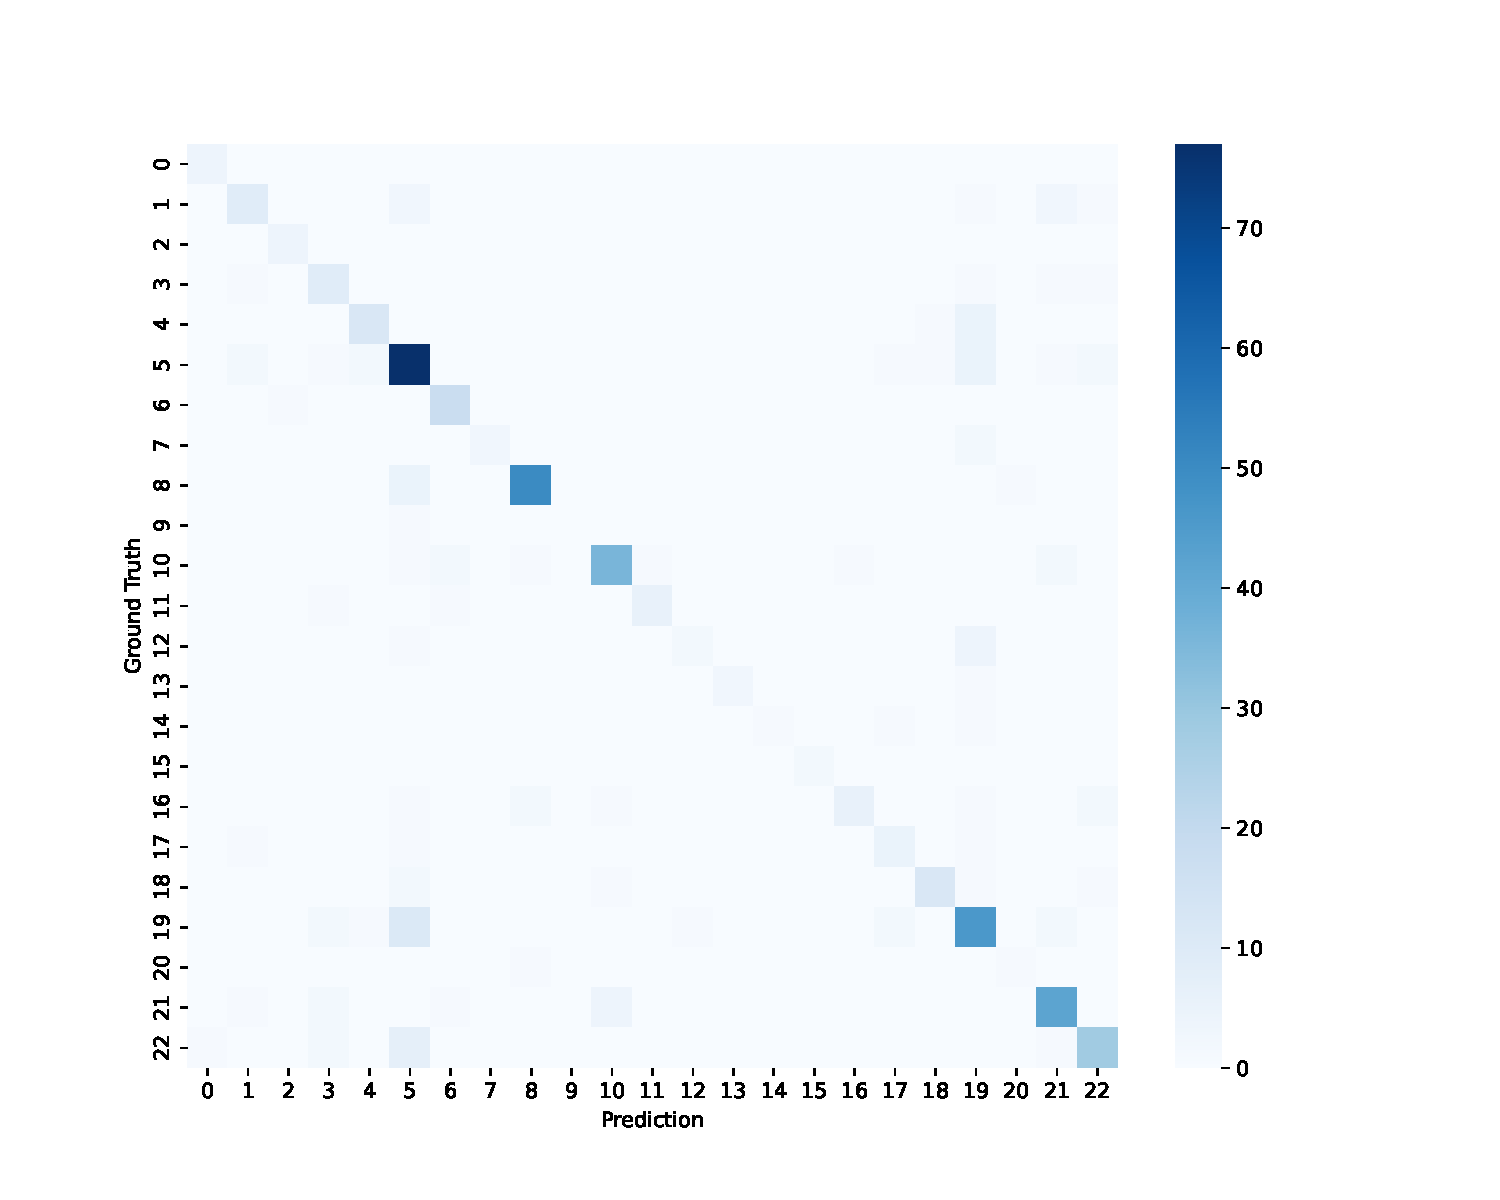
\includegraphics[width=\textwidth]{confusion_matrix_gnn.pdf}
        \caption{GCN模型}
    \end{subfigure}
    \caption{Baseline模型和GCN模型在测试集上的混淆矩阵}
    \label{tab:gcn_confusion}
\end{figure}

可以看到,GCN模型在测试集上的准确率明显高于Baseline模型。同时,相较于将许多实例错误的分类到第0类(Field Theory)的Baseline模型,GCN模型的混淆矩阵未见明显的异常。这说明我们的GCN模型对于Mathlib4的数学定理和证明能够根据图的结构学习出结点的一些特征,在学科分类任务上取得了较好的效果。

\section{结论}

本次实验通过分析和处理Mathlib4项目中的数学定理和证明数据,我们展示了如何使用不同的社群识别方法以及图神经网络进行数学概念的分类和依赖关系分析。实验中,我们首先进行了数据预处理,筛选并提取了数学定理和证明文件,构建了一个具有4910个节点和13858条边的有向图。在此基础上,我们使用谱聚类和SBM模型进行社群识别,并采用图神经网络进行半监督学习,以预测每个节点的学科类别。

我们的实验结果表明,谱聚类和SBM模型能够有效识别出Mathlib4中的社群结构,并且这些社群结构在一定程度上与学科分类有关,但不完全一致。这一发现提示我们,Mathlib4项目中数学概念的依赖关系不仅仅受到学科分类的影响,还可能受到其他因素如逻辑关系和数学理论的内在联系的影响,社群识别的算法正是能为我们提供这一新的视角。我们的谱聚类和SBM模型的modularity均达到0.614,显示出了较好的社群划分效果。

此外,图神经网络在本实验中表现出色,其在测试集上的分类准确率显著高于基于众数表决的基线模型,达到了76.58\%。这一结果强调了利用图结构信息进行节点特征学习的重要性和有效性,特别是在处理依赖关系复杂的数学定理和证明数据时。

总的来说,社群识别算法在探索图结构和揭示潜在社群关系方面具备较强优势,而图神经网络则更适合带有标签的任务,能够在半监督的分类任务中取得更高的性能和可解释性。两者在本实验中的结果相辅相成,共同揭示了Mathlib4数学定理依赖关系中的重要特征。